\documentclass[12pt,letterpaper]{article}
\usepackage{fullpage}
\usepackage[top=2cm, bottom=4.5cm, left=2.5cm, right=2.5cm]{geometry}
\usepackage{amsmath,amsthm,amsfonts,amssymb,amscd}
\usepackage{lastpage}
\usepackage{enumerate}
\usepackage{fancyhdr}
\usepackage{mathrsfs}
\usepackage{xcolor}
\usepackage{graphicx}
\usepackage{listings}
\usepackage{hyperref}
\usepackage{txfonts}
\usepackage{titlesec}

\usepackage{tikz}
\usetikzlibrary{trees}

\hypersetup{%
  colorlinks=true,
  linkcolor=blue,
  linkbordercolor={0 0 1}
}

% Edit these as appropriate
\newcommand\course{A\&D W5}
\newcommand\hwnumber{5}                  % <-- homework number
\newcommand\MyName{Simon Ganter} % <-- Your Name
 
\renewcommand\lstlistingname{Algorithm}
\renewcommand\lstlistlistingname{Algorithms}
\def\lstlistingautorefname{Alg.}

\setlength{\parindent}{0.0in}
\setlength{\parskip}{0.05in}

\titleformat{\section}[hang]{\normalfont\bfseries}{}{0pt}{} % Removes section numbers
\titleformat{\subsection}[hang]{\normalfont}{}{0pt}{} % Removes subsection numbers


\pagestyle{fancyplain}
\headheight 35pt
\lhead{\MyName{}}
\chead{\textbf{Ex Sheet \hwnumber}}
\rhead{\course \\ October 24, 2023}
\lfoot{}
\cfoot{}
\rfoot{\small\thepage}
\headsep 1.5em

\begin{document}

% Start solutions here
\section{\hwnumber.1 Sorting algorithms}
top left: Insertion Sort\\
top right: Bubble Sort\\
bottom left: Merge Sort \\
bottom right: Selection Sort\\

\section{\hwnumber.2 Guessing an interval}

\subsection{a)}
Prove that a strategy to win the game in 12 attempts doesn't exist.\bigbreak
\textbf{At most} means that it holds for worst cases.\\
The lower bound to find an element in a sorted array is defined by $O(\log{n})$.\\
If Bob \textit{would get} information to both of his integers after each attempt - he could tell it in max: $\lceil \log_{2}{200} \rceil = 8$ attempts.\bigbreak
\textbf{But: }The worst case for Bob is:\\
Alice selects her two values like: $a,\quad b = a+ 1$.\\
Now with this choice from Alice, Bob will never get information about his integers except if they are correct and he wins. Why? Because both of his values must be in between and there are no values in between an arbitrary int a and a + 1.\bigbreak
We note that now Bob can choose which ever strategy he want but for one guess of $a' \ and \ b'$ he will just know one pair $a', b'$. And since there are 199 of these (worst case) pairs he cannot have a strategy with which he wins in less or equal to 12 attempts.

\subsection{b)*}
As i showed in subsection a) also this is not possible.

\newpage
\section{5.3 Building a Heap}

\subsection{a) \textit{Prove that at most $O(\log{n})$ comparisons between keys are performed in the execution of Insert(H,k)}}
One of the heap conditions are: that every parent except for the the last one has exactly 2 children. So we know that our heap has a depth of: $\lceil \log_{2}{n} \rceil$\\
We now start creating a new node to the bottom layer of our heap. \\
The first iteration of the while loop compares the node and the parent node. \bigbreak
If our new node is smaller than we stop.\\
If not then we swap these two elements and move on to compare the next two nodes.\\
So the algorithm does one comparison for one layer.\bigbreak 
\textbf{The worst case }will be if the new node is the biggest element in the heap: then it has to get swapped all the way to the top. In each layer it get compared once with his parent. We know there are $\log{n}$ layers so the new node  would get $\log{n}$ times compared.\bigbreak
\textit{note: } The heap condition everywhere else than at the new node will be preserved through out this hole process. If the while loop finishes the heap is completely resorted. (prove follows in b) and c))

\subsection{b) \textit{$N_{stop}$ - Prove heap condition to be satisfied in the depth $N_{stop}$ or under}}
If N isn't the root node, we know that all other nodes on the level of N (also the potential sibling node) satisfy the heap condition, because we didn't change anything in there scope.\bigbreak
So we must show that the heap condition under the node itself satisfy the heap condition.\\
This can be easily shown as the node N was only swapped with the node above, whenever it was greater. Because we are working with a heap we know after a swap it will be the greatest node of all nodes underneath itself.\bigbreak
So we showed that the nodes \textbf{at the same level} (if they exist) won't have been, thus still satisfy the heap condition. The nodes \textbf{underneath} the node N are all strictly smaller than N because we only swapped with the parent node if it was strictly greater.

\newpage
\subsection{c) \textit{Prove heap condition to be satisfied above depth $N_{stop}$}}
\textbf{Invariant: } After iteration t the heap condition is satisfied for all levels strictly greater than depth $\log{n} - t$.\bigbreak
\textbf{Base Case: } t = 1\\
After the first iteration we (eventually) swapped N if it was greater than its parent.\\
The only node that eventually doesn't satisfy the heap condition is the swapped node N. This can be if it is smaller than its parent.\\
\textit{But} all nodes on the level 2 or higher still maintain the condition that they are either a root node, or smaller or equal to there parent node.\bigbreak
\textbf{Induction Hypothesis: } we assume that the property (the invariant) holds for some iterations j in the while loop.\bigbreak
\textbf{Induction Step. } t $\to$ t + 1\\
We know from our Hyp. that before iteration t + 1 the elements in depth $\log{n} - t - 1$ and above satisfied the heap condition.\\
Now with similar logic as before we can show that after a swap of N with its parent we only risk potentially the heap condition at depth $\log{n} - t -1 $\bigbreak
all nodes on the level t + 2 or higher maintain the condition that they are either a root node, or smaller or equal to there parent node. We never changed something to there parent node so they still have to have heap condition.\bigbreak

\textbf{Conclusion: } if the algorithm ends than either\\
\textit{is N the root node}\\
\textit{or N is smaller} than its parent node. Than:\\ 
We know from b) that in the end of the algorithm all nodes on the same level to N or less satisfy the heap condition.\\
No we can add from the proof by induction that the heap condition for the levels above also satisfy the heap condition.

\newpage
\section{5.4 Implementing abstract data types}

\subsection{a) implement the ADT stack}
with \textbf{linked lists} we could easily implement the data type stack like this\\
\textit{push:} we set the beginning link to the new element and from there add another link to the second element.\\
\textit{pop:} we follow the beginning link to the first element return it and set the beginning link to the second element.

\subsection{b) implement the ADT Queue}
\textit{enqueue:} we connect the new element to null and the last element of the list to the new one.\\
\textit{dequeue:} same as pop... we follow the beginning link to the first element return it and set the beginning link to the second element.

\newpage
\section{5.5 AVL trees}
\subsection{a) inserting keys 3, 8, 6, 5, 2, 9, 1, 0}
\textbf{inserting 3}

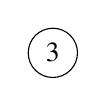
\begin{tikzpicture}[level/.style={sibling distance=60mm/#1}]
    \node [circle,draw] {3};
\end{tikzpicture}\\

\textbf{inserting 8}\\
\begin{tikzpicture}[level/.style={sibling distance=60mm/#1}]
    \node [circle,draw] {3}
      child {node [circle, draw]  {}}
      child {node [circle, draw]  {8}};
\end{tikzpicture}

\textbf{inserting 6}\\
\begin{tikzpicture}[level/.style={sibling distance=60mm/#1}]
    \node [circle,draw] {3}
      child {node [circle, draw]  {}}
      child {node [circle, draw]  {8}
            child {node [circle, draw]  {6}}
            child {node [circle, draw]  {}}
        }
        ;
\end{tikzpicture}

\textbf{right-left-rotation}\\
\begin{align*}
&\begin{tikzpicture}[level/.style={sibling distance=60mm/#1}]
    \node [circle,draw] {3}
      child {node [circle, draw]  {}}
      child {node [circle, draw]  {8}
            child {node [circle, draw]  {6}}
            child {node [circle, draw]  {}}
        }
        ;
\end{tikzpicture}
 \to \ right \ rot.
 \begin{tikzpicture}[level/.style={sibling distance=60mm/#1}]
    \node [circle,draw] {3}
      child {node [circle, draw]  {}}
      child {node [circle, draw]  {6}
            child {node [circle, draw]  {}}
            child {node [circle, draw]  {8}}
        }
        ;
\end{tikzpicture}\\
&\to \ left \ rot. 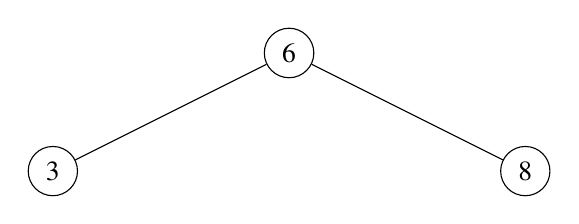
\begin{tikzpicture}[level/.style={sibling distance=60mm/#1}]
    \node [circle,draw] {6}
      child {node [circle, draw]  {3}}
      child {node [circle, draw]  {8}}
        ;
\end{tikzpicture}
\end{align*}

\newpage

\textbf{inserting 5}\\
\begin{tikzpicture}[level/.style={sibling distance=60mm/#1}]
    \node [circle,draw] {6}
      child {node [circle, draw]  {3}
          child {node [circle, draw]  {}}
          child {node [circle, draw]  {5}}
      }
      child {node [circle, draw]  {8}}
        ;
\end{tikzpicture}

\textbf{inserting 2}\\
\begin{tikzpicture}[level/.style={sibling distance=60mm/#1}]
    \node [circle,draw] {6}
      child {node [circle, draw]  {3}
          child {node [circle, draw]  {2}}
          child {node [circle, draw]  {5}}
      }
      child {node [circle, draw]  {8}}
        ;
\end{tikzpicture}

\textbf{inserting 9}\\
\begin{tikzpicture}[level/.style={sibling distance=60mm/#1}]
    \node [circle,draw] {6}
      child {node [circle, draw]  {3}
          child {node [circle, draw]  {2}}
          child {node [circle, draw]  {5}}
      }
      child {node [circle, draw]  {8}
            child {node [circle, draw]  {}}
            child {node [circle, draw]  {9}}
      }
        ;
\end{tikzpicture}

\textbf{inserting 1}\\
\begin{tikzpicture}[level/.style={sibling distance=60mm/#1}]
    \node [circle,draw] {6}
      child {node [circle, draw]  {3}
          child {node [circle, draw]  {2}
            child {node [circle, draw]  {1}}
            child {node [circle, draw]  {}}
          }
          child {node [circle, draw]  {5}}
      }
      child {node [circle, draw]  {8}
            child {node [circle, draw]  {}}
            child {node [circle, draw]  {9}}
      }
        ;
\end{tikzpicture}

\newpage

\textbf{inserting 0}\\
\begin{tikzpicture}[level/.style={sibling distance=60mm/#1}]
    \node [circle,draw] {6}
      child {node [circle, draw]  {3}
          child {node [circle, draw]  {2}
            child {node [circle, draw]  {1}
                child {node [circle, draw]  {0}}
                child {node [circle, draw]  {}}
            }
            child {node [circle, draw]  {}}
          }
          child {node [circle, draw]  {5}}
      }
      child {node [circle, draw]  {8}
            child {node [circle, draw]  {}}
            child {node [circle, draw]  {9}}
      }
        ;
\end{tikzpicture}

\textbf{left-left-rotation}\\
We see the state before above\\
$\to \ left \ rot.$
\begin{tikzpicture}[level/.style={sibling distance=60mm/#1}]
    \node [circle,draw] {6}
      child {node [circle, draw]  {3}
          child {node [circle, draw]  {1}
            child {node [circle, draw]  {0}}
            child {node [circle, draw]  {2}}
          }
          child {node [circle, draw]  {5}}
      }
      child {node [circle, draw]  {8}
            child {node [circle, draw]  {}}
            child {node [circle, draw]  {9}}
      }
        ;
\end{tikzpicture}

\newpage
\subsection{b) Deleting 6, 12, 7, 4}

\begin{tikzpicture}[level/.style={sibling distance=60mm/#1}]
    \node [circle,draw] {7}
      child {node [circle, draw]  {2}
          child {node [circle, draw]  {0}
          }
          child {node [circle, draw]  {4}
            child {node [circle, draw]  {3}}
            child {node [circle, draw]  {6}}
          }
      }
      child {node [circle, draw]  {9}
            child {node [circle, draw]  {}}
            child {node [circle, draw]  {12}}
      }
        ;
\end{tikzpicture}

\textbf{delete 6}\\
\begin{tikzpicture}[level/.style={sibling distance=60mm/#1}]
    \node [circle,draw] {7}
      child {node [circle, draw]  {2}
          child {node [circle, draw]  {0}
          }
          child {node [circle, draw]  {4}
            child {node [circle, draw]  {3}}
            child {node [circle, draw]  {}}
          }
      }
      child {node [circle, draw]  {9}
            child {node [circle, draw]  {}}
            child {node [circle, draw]  {12}}
      }
        ;
\end{tikzpicture}

\textbf{delete 12}\\
\begin{tikzpicture}[level/.style={sibling distance=60mm/#1}]
    \node [circle,draw] {7}
      child {node [circle, draw]  {2}
          child {node [circle, draw]  {0}
          }
          child {node [circle, draw]  {4}
            child {node [circle, draw]  {3}}
            child {node [circle, draw]  {}}
          }
      }
      child {node [circle, draw]  {9}
            child {node [circle, draw]  {}}
            child {node [circle, draw]  {}}
      }
        ;
\end{tikzpicture}

\newpage
\textbf{left-right-rotation}\\
\begin{tikzpicture}[level/.style={sibling distance=60mm/#1}]
    \node [circle,draw] {7}
      child {node [circle, draw]  {2}
          child {node [circle, draw]  {0}
          }
          child {node [circle, draw]  {4}
            child {node [circle, draw]  {3}}
            child {node [circle, draw]  {}}
          }
      }
      child {node [circle, draw]  {9}
            child {node [circle, draw]  {}}
            child {node [circle, draw]  {}}
      }
        ;
\end{tikzpicture}\\
$\to left-rot.$
\begin{tikzpicture}[level/.style={sibling distance=60mm/#1}]
    \node [circle,draw] {7}
      child {node [circle, draw]  {4}
          child {node [circle, draw]  {2}
            child {node [circle, draw]  {0}}
            child {node [circle, draw]  {}}
          }
          child {node [circle, draw]  {3}
          }
      }
      child {node [circle, draw]  {9}
      }
        ;
\end{tikzpicture}\\
$\to right-rot.$
\begin{tikzpicture}[level/.style={sibling distance=60mm/#1}]
    \node [circle,draw] {4}
      child {node [circle, draw]  {2}
          child {node [circle, draw]  {0}
          }
          child {node [circle, draw]  {3}
          }
      }
      child {node [circle, draw]  {7}
            child {node [circle, draw]  {}}
            child {node [circle, draw]  {9}}
      }
        ;
\end{tikzpicture}

\newpage

\textbf{delete 7}\\
\begin{tikzpicture}[level/.style={sibling distance=60mm/#1}]
    \node [circle,draw] {4}
      child {node [circle, draw]  {2}
          child {node [circle, draw]  {0}
          }
          child {node [circle, draw]  {3}
          }
      }
      child {node [circle, draw]  {}
            child {node [circle, draw]  {}}
            child {node [circle, draw]  {9}}
      }
        ;
\end{tikzpicture}\\
$\to $ take smallest element of the right arm
\begin{tikzpicture}[level/.style={sibling distance=60mm/#1}]
    \node [circle,draw] {4}
      child {node [circle, draw]  {2}
          child {node [circle, draw]  {0}
          }
          child {node [circle, draw]  {3}
          }
      }
      child {node [circle, draw]  {9}
      }
        ;
\end{tikzpicture}

\textbf{delete 4}\\
\begin{tikzpicture}[level/.style={sibling distance=60mm/#1}]
    \node [circle,draw] {}
      child {node [circle, draw]  {2}
          child {node [circle, draw]  {0}
          }
          child {node [circle, draw]  {3}
          }
      }
      child {node [circle, draw]  {9}
      }
        ;
\end{tikzpicture}\\
$\to $ take smallest element of the right arm
\begin{tikzpicture}[level/.style={sibling distance=60mm/#1}]
    \node [circle,draw] {9}
      child {node [circle, draw]  {2}
          child {node [circle, draw]  {0}
          }
          child {node [circle, draw]  {3}
          }
      }
      child {node [circle, draw]  {}
      }
        ;
\end{tikzpicture}\\
$\to $ right rot.
\begin{tikzpicture}[level/.style={sibling distance=60mm/#1}]
    \node [circle,draw] {2}
      child {node [circle, draw]  {0}
      }
      child {node [circle, draw]  {9}
          child {node [circle, draw]  {3}
          }
          child {node [circle, draw]  {}
          }
      }
        ;
\end{tikzpicture}



\end{document}
